%%%%%%%%%%%%%%%%%%%%%%%%%%%%%%%%%%%%%%%%%%%%%%%%%%%%%%%%%%%%%%%%%%%%%%%%%%%
%% This file is part of the book
%%
%% Algorithmic Graph Theory
%% http://code.google.com/p/graph-theory-algorithms-book/
%%
%% Copyright (C) 2009--2011 Minh Van Nguyen <nguyenminh2@gmail.com>
%%
%% See the file COPYING for copying conditions.
%%%%%%%%%%%%%%%%%%%%%%%%%%%%%%%%%%%%%%%%%%%%%%%%%%%%%%%%%%%%%%%%%%%%%%%%%%%

\documentclass{article}

\usepackage{pgfplots}
\usetikzlibrary{external}
\tikzexternalize{eccentricity-distribution}

\begin{document}

\begin{figure}
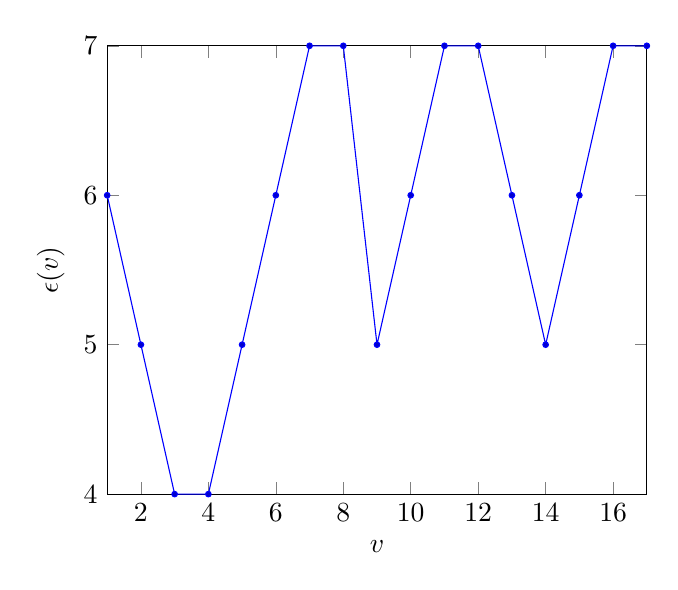
\begin{tikzpicture}
[every mark/.append style={scale=0.5}]
\begin{axis}[%
  enlargelimits=false,%
  xlabel=$v$,%
  ylabel=$\epsilon(v)$%
]
\addplot+[sharp plot] coordinates
{
  (1, 6)   (2, 5)   (3, 4)   (4, 4)   (5, 5)
  (6, 6)   (7, 7)   (8, 7)   (9, 5)   (10, 6)
  (11, 7)  (12, 7)  (13, 6)  (14, 5)  (15, 6)
  (16, 7)  (17, 7)
};
\end{axis}
\end{tikzpicture}
\end{figure}

\end{document}
